\section{Sensibility Testbed Design}\label{sec-design}

This section describes the design of the Sensibility Testbed. 
%On one hand, Sensibility Testbed manages how device owners make their
%devices accessible to the research community. On the other hand,
%it offers technical resources to researchers that allow them to
%securely collect data from remote mobile devices. 
We start with
an overview of the testbed infrastructure (Section~\ref{sec-overview}), 
and a description of each testbed component 
(Section~\ref{sec-component}), then finally a discussion of how all the 
components work together to assist experimenters' experimentation,
and protect device owners' personal information 
(Section~\ref{sec-scenario}).


\subsection{Overview}\label{sec-overview}

In Sensibility Testbed, the data blurring 
mechanism is implemented as blurring layers, each layer acting as a 
reference monitor in a sandbox~\cite{ref} that enforces an access 
control policy over sensor access. Using the sandboxing 
technique in our prior work~\cite{cappos2010retaining}, we can 
interject code to implement privacy policies and control what 
happens with the data gathered on the device. A sensor access 
policy can (1) reduce 
the precision of the raw sensor data returned from a device, such
as returning the location of a nearest city rather than the device's exact location; (2) restrict 
the frequency of accessing a sensor, such as the polling rate of 
accelerometer, to avoid password inferring; and (3) disable  
access to a certain sensor in sensitive situations, such as 
turning off camera when a device is at residential or work areas.
The last policy is our ongoing work. This paper mainly addresses
the first two types of policies. 

%\subsubsection{Interacting Parties}\label{sec-parties}
In Sensibility Testbed, there are three types of interacting
parties, as shown in Figure~\ref{fig-arch}: mobile devices 
owned by ordinary people, with our app installed; a 
clearinghouse server that discovers and configures
participating devices; and experimenters who want to run
experiments on mobile devices. 

\begin{figure}
\center{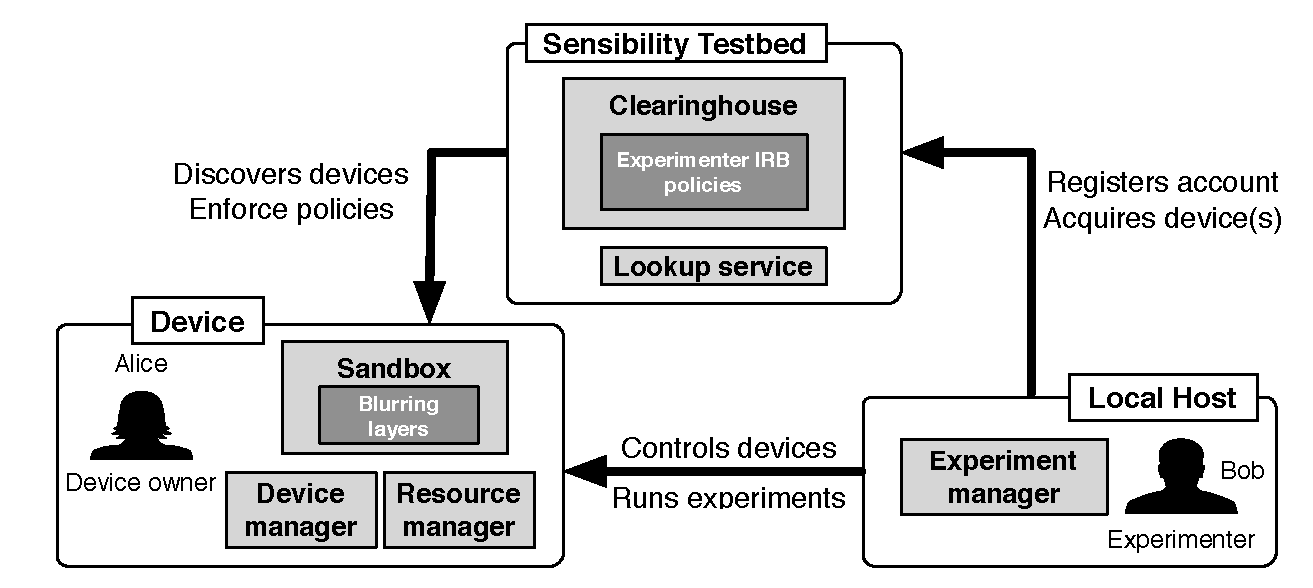
\includegraphics[width=\columnwidth]{figs/arch.pdf}}
%\vspace*{-20pt}
\caption{\small Sensibility Testbed architecture. \label{fig-arch}}
\end{figure}

Mobile devices
provide resources and data for researchers to use in their
experiments. In order to perform safe experiments on mobile
devices, a researcher must provide to the clearinghouse server
the IRB policies from his institute for accessing devices 
(Section~\ref{sec-ch}). \yanyan{need a screenshot} These 
policies restrict what and how data can be accessed by the 
researcher. The
clearinghouse server helps the researcher acquire and manage
devices, and also codifies the policies specified by the
researcher's IRB into data blurring layers that are enforced on
mobile devices (Section~\ref{sec-policy}). Such a process can protect device
owners' personal information. After obtaining remote sandboxes
and having IRB policies in place, researchers can perform
experiments on the devices using their credentials assigned by
the clearinghouse. Researchers' code runs in a sandbox on any
remote device that isolates the code from the rest of the device
host system (Section~\ref{sec-repy}). To control the execution of 
code, the researcher uses a local machine to manage the 
experiments via an experiment manager. This tool can deploy 
and run experiments in sandboxes on remote devices that are 
acquired through the clearinghouse (Section~\ref{sec-emt}).

%\subsubsection{Enforcing IRB Approved Policies}


\subsection{Testbed Components}\label{sec-component}

The components of the Sensibility Testbed are shown in Figure~\ref{fig-arch}.
They are central to the operation of the testbed. 
In this section, we describe the function of each component: the
secure sandbox~\cite{cappos2010retaining}, clearinghouse~\cite{ch}, 
and experiment manager.

\subsubsection{Secure Sandbox}\label{sec-repy}

%In Sensibility Testbed, all experiments execute in a secure 
%sandbox on the end devices.
%Experimenters' code executes in a sandbox that isolates the 
%experiment code from the device host system. 
Sensibility Testbed uses a sandbox called Repy (Restricted 
Python)\footnote{\scriptsize This is the 
same security-reviewed sandbox~\cite{cappos2010retaining} used in
our prior work, the Seattle testbed~\cite{seattle}. This sandbox
mitigates the impact of bugs in experimenter code.}, which 
provides security isolation on mobile devices.
%Instead of developing full-fledged Android apps, all 
%experiments in Sensibility Testbed are written in a language
%similar to Python, and run in a secure %Python-based
Repy has a small, self-contained kernel as its trusted 
computing base (TCB). %unprivileged libraries and experiment code. 
Every system call in the TCB is strictly 
sanitized to preserve consistent behavior across difference OSes, 
and to avoid uncommon corner cases that can be exploited. 
Furthermore, since the TCB is small (about 8,000 lines of code), it is 
less likely to have a kernel exploit than other more complex kernels. 
As a result, any vulnerability in an experiment 
%can at most cause compromise in the unprivileged portion of the sandbox, 
cannot escape the sandbox and perform malicious actions to 
the device system. The Repy sandbox also exposes a Python-like 
programming language interface~\cite{repyv2} to experiment code 
for accessing resources on a device. For more than six years, the
sandbox has been used to run experiments as part of a network research 
testbed~\cite{seattle}, and there has been no report of security 
breaches or operational fault. 

In addition to security isolation,
%The sandbox exposes a programming 
%interface to experimenter programs to access 
%resources on the device. 
the sandbox provides performance isolation by
%by using OS hooks to monitor and control the amount of 
%CPU and memory used by a sandboxed program. To restrict 
%other resources, such as network and disk I/O, the sandbox 
interposition on system calls~\cite{garfinkel2003traps} that 
use resources, such as network and disk I/O, and preventing 
or delaying the execution of these calls if they exceed 
their configured quota. 
%As a result, this sandbox limits 
%what a sandboxed program can do. For example, 
Reading from and writing to the file system can
only occur in a per-experiment directory; sending and receiving
data via the network interface cannot exceed a configured rate;
CPU, memory and battery consumption cannot exceed a limit, etc.
Therefore, the sandbox isolates the experiment program from 
the rest of the device. Due to this isolation, different experimenters
can have access to different sandboxes on the same device,
and each sandbox is isolated from one another.

To install the sandbox on a device, a device owner downloads 
our Sensibility Testbed app from the Google Play Store \cite{sensibility-app}.
The app displays a consent form, which the device owner must 
agree to before the installation. If the device owner gives his
consent, the device will be installed with the Repy sandbox, the native Android code to 
start or stop the sandbox, and an interface to communicate with the testbed 
infrastructure, particularly the clearinghouse (described below). 
By agreeing to our general usage policy, device 
owners of different ages, from different countries, with different
background need only to opt in \textit{once} to our testbed as 
volunteers (during the time of app installation). An experimenter 
who wants to conduct a research experiment 
%requests devices through our clearinghouse, which assigns 
%them devices from a set of available resources. As a result, 
%the researcher
does not need to get consent from each subject for each individual
experiment. The testbed thus reduces the burden from both the 
device owners and experimenters. 

However, the current Repy sandbox does not include calls to access sensors. 
%To obtain the sensor data, we need to extend the sandbox. 
The extended Repy sandbox that allows sensor access  
will be described in Section~\ref{sec-repy-ext}.
More importantly, the extended sandbox allows us to change the 
behavior of its Python-like programming interface, and control the 
data gathered from the device. 
%For  an experiment
%that involves GPS location, a privacy policy might restrict the
%level of data granularity available to the experiment. For example, it can
%obfuscate GPS location such that it only identifies the center
%of the city that the device is located in, rather than the exact
%location. Using the same technique, 
To illustrate, the IP address of a device may be anonymized, 
the frequency to access GPS location can be constrained, and 
access to camera can be disabled, and so on. 
%Such privacy protection is a contribution of Sensibility Testbed, 
%which does not exist in any prior work. 
The details of policy implementation are presented in 
Section~\ref{sec-layer} and \ref{sec-nanny}.

\subsubsection{Clearinghouse}\label{sec-ch}
The clearinghouse~\cite{ch} is a testbed server that keeps 
track of devices and mediates experimenter access to the 
available devices. It allows experimenters to register 
accounts and share access to a common pool of devices.
It does so by looking up available devices, and assigning
them to researcher's experiment account upon request 
(details in Section~\ref{sec-acquire-run}). 
Its key role is to facilitate device sharing, 
which relieves individual experimenters from repeatedly 
recruiting devices for each experiment.

The clearinghouse
plays an intermediate role between the experimenter and 
the device owner.
As described in Section~\ref{sec-overview}, when an 
experimenter registers at the clearinghouse, he
needs to provide his IRB policies. These policies ensure that
the researcher cannot conduct experiments to access data that
extend beyond the experiment policy. The clearinghouse 
translates and codifies each policy, and instructs the 
sandboxes on remote devices to implement these policies. 
When experiment code is running in the sandbox, the 
policies will be applied to restrict %the precision of sensor 
%data or the frequency to access 
sensor access. This Sensibility Testbed
clearinghouse protocol for research plays a central role in
easing the device recruitment and experiment setup for experimenters, 
and ensures the enforcement
of privacy policy\footnote{\scriptsize The Sensibility Testbed Clearinghouse
protocol for research with human subjects has been approved by
the IRB at New York University (IRB \# 15-10751).}. 

\subsubsection{Experiment Manager}\label{sec-emt}

To run code remotely on mobile devices, an experimenter uses an
experiment manager from his local machine 
%which contains Bob's private key, \path{key.bob-priv}, 
to access the sandboxes on the remote devices under his control. 
This experiment manager is a light-weight command line 
console~\cite{demo-kit} that allows direct access from the 
experimenter's local machine to a set of remote devices. 
The clearinghouse is not involved when an experimenter deploys 
an experiment and runs the code, and it does not store any
data on the experimenter's behalf. After collecting the data he needs, the
experimenter can use the experiment manager to download data from the remote devices. 
Alternatively, the experimenter can set up his own server to store all 
the data\footnote{\scriptsize
If an experimenter stores data at his own server, he must use protective
measures to ensure that the data sent from the mobile devices is
properly encrypted, and the server storage cannot be tampered
with by any other parties. For example, the experimenter needs to register
his server by providing the server's certificate and URL to our
clearinghouse. The clearinghouse then instructs the devices
accessible to the experimenter that all the sensor data collected should be
sent to this server. The sandboxes on these devices then issue
\texttt{HTTPS POST} using the server's certificate, and send encrypted
data to the experimenter's server. After the data is collected, how to store
the data securely is mandated by the experimenter's IRB.}, or use a data 
store service we provide (a service called Sensevis~\cite{sensevis}, 
not shown in Figure~\ref{fig-arch}).

\smallskip
In summary, 
%Prior to running an experiment on Sensibility Testbed, a
%experimenter first fills out a form in plain text to describe the
%purpose of the research experiment. This experiment description
%is created at the Sensibility Testbed clearinghouse
%where the researcher indicates the type of data to be collected,
%how that data will be used and stored, and so on. 
%
%Once this information is collected from the researcher, the
%clearinghouse automatically generates a set of blurring layers
%that implements the experiment policy (Section~\ref{sec-policy}). In
%Sensibility Testbed, researchers can collect data from the
%sensors on the device, such as GPS, Bluetooth, battery
%information, accelerometer, light, and orientation,
%etc. The blurring layers we provide consist of
%data access restrictions, created in accordance with
%researcher's experiment description, by using the Sensibility
%Testbed's sandboxing technique 
%(Section~\ref{sec-repy})~\cite{cappos2010retaining}. These restrictions ensure that
%the researcher cannot conduct experiments to access data that
%extend beyond the experiment policy. 
%
%This Sensibility Testbed
%clearinghouse protocol for research plays a central role in
%easing the approval process of IRB, and ensures the enforcement
%of privacy policy\footnote{The Sensibility Testbed Clearinghouse
%protocol for research with human subjects has been approved by
%the IRB at New York University. \yanyan{might need a link to
%your approval letter or ref number}}. 
using Sensibility Testbed, device owners' privacy is protected
from any inadvertent or malicious attempt, and experimenters 
are able to go through a streamlined process of device 
recruitment and experiment setup.

%the device owners do not need to give consents 
%multiple times, to each project of each researcher. 
In the following, we present several use cases to
demonstrate how device owners opt in as volunteers, and how
researchers do experiments on devices without compromising device
owners' privacy.

\subsection{Testbed Scenarios}\label{sec-scenario}
\yanyan{should this section go after policies?}
To demonstrate how Sensibility Testbed lowers the barriers for
researchers to perform research experiments on mobile devices,
and protects device owners' privacy, this section will go
through several scenarios. In these scenarios, a smartphone owner, Alice,
participates in the testbed; an experimenter, Bob, runs code on
Sensibility Testbed using Alice's smartphone, among other
devices. Specifically, Bob wants to know the cellular service
quality in major cities. As such, he needs location information
of individual devices, their cellular service provider, network
type (3G, 4G, LTE, etc.), and signal strength.

Note that in Sensibility Testbed, there are two types of keys. A device
owner has an \textit{identification key} to identify the app installed on a 
device. An experimenter has a pair of public/private \textit{authentication 
keys} to authenticate the experimenter with the clearinghouse and 
the set of devices that he has access to.

\subsubsection{Smartphone Owner Participates in the Testbed}
\label{sec-owner-participate}

When Alice, a smartphone owner, decides to participate in
Sensibility Testbed, she first downloads our Sensibility Testbed
app~\cite{sensibility-app}. %which currently supports Android devices.
This app contains a testbed key \path{key.sensibility} used for 
device discovery (similar to a device owner's identification key). 
%the Repy sandbox (Section~\ref{sec-repy}), 
%and native Android code to handle user interaction, communicate 
%with the clearinghouse, and so on. 
Before installation, the app displays a
consent form to Alice \yanyan{cite link}, where she can review
the testbed's general usage policy \yanyan{cite link}. If Alice
agrees to the terms and policy, the app will be installed on her
device. When the app is started, Alice's device can be
discovered by the clearinghouse (Section~\ref{sec-acquire-run}). 
To keep track of Alice's device, the
clearinghouse uses a database that stores her device's unique
identification key, \path{key.alice}, generated during installation 
(Section~\ref{sec-acquire-run}). This key is not associated with Alice's or her
device's identity, but only the app's installation on the device. If
Alice uninstalls the Sensibility app, \path{key.alice} is
deleted at the clearinghouse, which effectively unlinks
her device from any metadata stored on the clearinghouse.
Instead of uninstalling, Alice may also choose to opt out of
individual experiments.

\subsubsection{Researcher Provides IRB
Policies}\label{sec-irb-policy}

To run code on Sensibility Testbed, experimenter Bob provides a
set of detailed IRB policies from his institution. The process of how
Bob obtains such policies is described in Section~\ref{sec-irb-policies}.
The policies specify 
what data can be accessed by a research experiment, at which 
granularity or frequency such data can be accessed, how data 
should be securely stored, and so on. \yanyan{cite register 
experiment website url.}
For example, Bob's experiment can (1) read location information
from devices at the granularity of a city, (2) read accurate
cellular signal strength and network type, but not allow access to 
information about cell IDs, and (3) get location and
cellular network data updates every 10 minutes. 
%Bob submits an
%experiment description for these requirements, which the
%clearinghouse will codify into policies that are later enforced
%on remote mobile devices (Section~\ref{sec-ch}).

After submitting his IRB policies, Bob obtains an account at the
clearinghouse, and his authentication keys. 
%\path{bob.public} and \path{bob.private}.

\subsubsection{Researcher Acquires Device(s) and Runs an
Experiment}\label{sec-acquire-run}

%The above clearinghouse protocol ensures the enforcement of data
%access policies. Additionally, 
To perform an experiment, the clearinghouse first needs to 
acquire and assign devices to Bob's experiment account. 
Recall that a testbed-specific key, \path{key.sensibility}, is distributed
with the Sensibility Testbed app downloaded and installed by device
owners (Section~\ref{sec-owner-participate}). When the app is started, 
Alice's device contacts a lookup service to advertise itself to Sensibility 
Testbed using \path{key.sensibility}. A lookup service is a distributed
key-value store, such as a DHT, that allows one to retrieve values 
associated with keys and to associate keys with values. 
The clearinghouse periodically queries the lookup service to
discover any new devices. Once Alice's device is discovered, the
clearinghouse obtains its identification key \path{key.alice} generated
during installation, and stores this key in a database. 

%\yanyan{Albert thinks this is too much detail.}
At this moment,  Bob has obtained an account with the clearinghouse 
(Section~\ref{sec-irb-policy}).
%and is assigned a pair of public and 
%private keys, \path{key.bob-pub} and \path{key.bob-priv}, by the
%clearinghouse. 
When Bob requests a device, and the clearinghouse
happens to find that Alice's device is available, the
clearinghouse first 
%adds Bob's public key, \path{key.bob-pub}, to
%the sandbox on Alice's device. This indicates that Bob is
%authorized to use this sandbox on Alice's device, and 
assigns Alice's device to Bob's experiment account, then instructs 
the sandbox on Alice's device to add Bob's policies by preloading
a set of blurring layer code.
%Bob writes his experiment 
%code in the Python-like language supported by our secure sandbox.
%The following is a snipet of code that gets location coordinates 
%from a device:

Next, Bob needs to upload his code to Alice's device and 
run the experiment. When he accesses the device through
the experiment manager, the sandbox on Alice's device 
applies the data access policies loaded by the clearinghouse: For policy (1) in
Section~\ref{sec-irb-policy}, the sandbox blurs the location
information returned from Alice's phone down to the coordinates
of the nearest city; for policy (2), the sandbox blocks the
access to cell IDs; for policy (3), the sandbox limits the rate
of GPS location and cellular network queries from Bob's
experiment to one in every 10 minutes.

\subsection{IRB and Sensibility Testbed}\label{sec-irb-policies}

In the domain of IRB, Alice and Bob are the participating subject, and 
a researcher who conducts a research study on the subject, respectively.
In order to obtain an IRB approval, Bob first has to fill out an experiment
registration form \yanyan{cite url or show screenshot} at the 
Sensibility clearinghouse, where
there is a list of available sensors, and each of their required accuracy 
and access frequency. Aftering filling out this form, Bob uses it as 
a template form to submit and apply for IRB approval at his institution. 
This form serves as a reference document, along with details about 
Sensibility Testbed, to reduce Bob's burden. 

After Bob's application is submitted, his IRB may disagree with 
Bob's experiment requirement. For example, Bob wants to access cell 
IDs in cellular networks, but his IRB disallows such data access. Bob then
revises his experiment requirement, obtains his IRB approval, and
submits the revised experiment registration form to our clearinghouse. Finally, the clearinghouse
parses the registration form, extracts each data accuracy and access 
frequency approved by Bob's IRB, and supplies them as input parameters to
the blurring layers that will be instantiated at Alice's device. The clearinghouse
has a default set of blurring layers for each sensor, each have the 
sensor's accuracy and access frequency as parameters. The details about
how each policy is implemented will be introduced in 
Section~\ref{sec-policy}.

\textbf{Sensibility Testbed's default policies.}
Note that Bob cannot request access to all sensors at any rate
even if his IRB approves such a policy. The Sensibility Testbed's
own IRB allows a set of default policies to access sensors in a
way that is low risk, \yanyan{cite}and for which access can be pre-approved with the
researcher's local IRB. However, Sensibility Testbed does not
provide unfettered access to all sensors. Access to sensors of
higher risk, e.g., the policies that request restricted sensor data, 
or at higher frequencies than our default policies, 
needs to go through the Sensibility Testbed's IRB,
in addition to the researcher's IRB. In most cases, we expect
that a researcher need only go through their local IRB to get
the sensor access they need for their experiment. After
providing his IRB policies, Bob next can obtain an experiment
account and request a number of devices from our clearinghouse.